\documentclass[]{book}

%These tell TeX which packages to use.
\usepackage{array,epsfig}
\usepackage{amsmath}
\usepackage{amsfonts}
\usepackage{amssymb}
\usepackage{amsxtra}
\usepackage{amsthm}
\usepackage{mathrsfs}
\usepackage{color}
\usepackage[spanish, mexico]{babel}
\usepackage[utf8]{inputenc}
\usepackage{hyperref}

%Here I define some theorem styles and shortcut commands for symbols I use often
\theoremstyle{definition}
\newtheorem{defn}{Definition}
\newtheorem{thm}{Theorem}
\newtheorem{cor}{Corollary}
\newtheorem*{rmk}{Remark}
\newtheorem{lem}{Lemma}
\newtheorem*{joke}{Joke}
\newtheorem{ex}{Example}
\newtheorem*{sol}{Solution}
\newtheorem{prop}{Proposition}

\newcommand{\lra}{\longrightarrow}
\newcommand{\ra}{\rightarrow}
\newcommand{\surj}{\twoheadrightarrow}
\newcommand{\graph}{\mathrm{graph}}
\newcommand{\bb}[1]{\mathbb{#1}}
\newcommand{\Z}{\bb{Z}}
\newcommand{\Q}{\bb{Q}}
\newcommand{\R}{\bb{R}}
\newcommand{\C}{\bb{C}}
\newcommand{\N}{\bb{N}}
\newcommand{\M}{\mathbf{M}}
\newcommand{\m}{\mathbf{m}}
\newcommand{\MM}{\mathscr{M}}
\newcommand{\HH}{\mathscr{H}}
\newcommand{\Om}{\Omega}
\newcommand{\Ho}{\in\HH(\Om)}
\newcommand{\bd}{\partial}
\newcommand{\del}{\partial}
\newcommand{\bardel}{\overline\partial}
\newcommand{\textdf}[1]{\textbf{\textsf{#1}}\index{#1}}
\newcommand{\img}{\mathrm{img}}
\newcommand{\ip}[2]{\left\langle{#1},{#2}\right\rangle}
\newcommand{\inter}[1]{\mathrm{int}{#1}}
\newcommand{\exter}[1]{\mathrm{ext}{#1}}
\newcommand{\cl}[1]{\mathrm{cl}{#1}}
\newcommand{\ds}{\displaystyle}
\newcommand{\vol}{\mathrm{vol}}
\newcommand{\cnt}{\mathrm{ct}}
\newcommand{\osc}{\mathrm{osc}}
\newcommand{\LL}{\mathbf{L}}
\newcommand{\UU}{\mathbf{U}}
\newcommand{\support}{\mathrm{support}}
\newcommand{\AND}{\;\wedge\;}
\newcommand{\OR}{\;\vee\;}
\newcommand{\Oset}{\varnothing}
\newcommand{\st}{\ni}
\newcommand{\wh}{\widehat}

%Pagination stuff.
\setlength{\topmargin}{-.3 in}
\setlength{\oddsidemargin}{0in}
\setlength{\evensidemargin}{0in}
\setlength{\textheight}{9.in}
\setlength{\textwidth}{6.5in}
\setlength{\itemsep}{0.45in}
\pagestyle{empty}



\begin{document}

\begin{center}
{\huge Implementación de Métodos Computacionales TC2037}\\[1.5ex]
{\large \textbf{Tarea 04 -- Lenguajes Regulares}\\[1.5ex] %You should put your name here
} %You should write the date here.
\end{center}

\section*{Autómatas Finitos Deterministas}

Con ayuda de Automaton Simulator (\url{https://automatonsimulator.com/}), generen \textdf{un DFA correcto y completo} para cada uno de los lenguajes especificados.
Además, incluyan \textdf{una expresión regular en formato PCRE} para cada uno.

\bigskip

\begin{enumerate}
	\itemsep3.5ex
	\item El lenguaje de las palabras en $\{a,b\}^*$ que contienen exactamente 2 $a$s.
	\begin{itemize}
		\item Se aceptan: $aa, baa, aba, bababb, \dots$
		\item No se aceptan: $\varepsilon , a, b, aaa, bbbb, \dots$
	\end{itemize}
	
	\item El lenguaje de los números binarios que si tienen un solo dígito $0$, debe ser el último dígito del número. (La palabra vacía no es un número binario).
	\begin{itemize}
		\item Se aceptan: $0, 10, 11, 001, 0101, 1110, 1000, \dots$
		\item No se aceptan: $\varepsilon , 01, 1101, 110111, 011, \dots$
	\end{itemize}

	\item El lenguaje de las palabras en $\{a, b\}^*$ que contienen la subcadena $aa$ y contienen la subcadena $bb$.
	\begin{itemize}
		\item Se aceptan: $aabb, bbbaa, aababb, abaababba, \dots$
		\item No se aceptan: $\varepsilon , a, b, abb, aab, ababa, \dots$
	\end{itemize}

	\item El lenguaje de las palabras en $\{0,1 \}^*$ que contienen un número par de $0$s o un número impar de $1$s.
	\begin{itemize}
		\item Se aceptan: $\varepsilon , 1, 11, 00, 1011, 10101, 11100, \dots$
		\item No se aceptan: $0, 011, 11011, 01010, \dots$
	\end{itemize}

	\item El lenguaje de las palabras en $\{a, b\}^*$ que si terminan con $b$ entonces tienen una sola $b$, y si empieza con $a$ entonces tiene al menos otra $a$.
	\begin{itemize}
		\item Se aceptan: $\varepsilon , b, aab, aa, ba, bba, ababa, \dots$
		\item No se aceptan: $a, ab, bb, abb, baaab, \dots$
	\end{itemize}
\end{enumerate}

\section*{Entregables}

\begin{minipage}{0.1\linewidth}
	\centering
	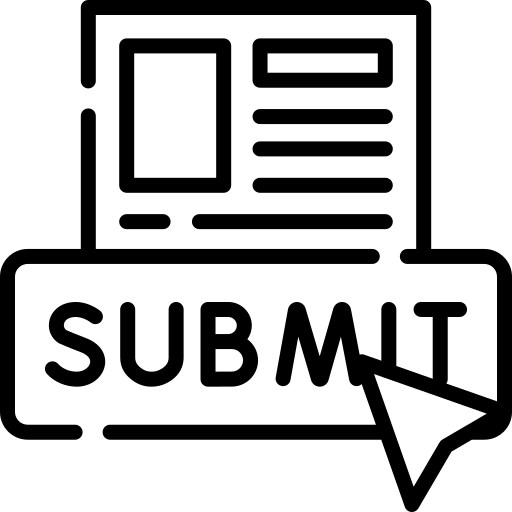
\includegraphics[scale = 0.06]{../img/submit}
\end{minipage}%
\begin{minipage}{0.85\linewidth}
	Al finalizar, enumeren y guarden cada uno de los DFAs generados (\texttt{.json} si usaron Automaton Simulator), y súbanlos en una carpeta comprimida (\texttt{.zip}) con el nombre\\$M_1$-$M_2$\texttt{-hw04.zip}, donde $M_i$ es el número de matrícula del $i$-ésimo miembro de su equipo.
	Con que uno de los integrantes suba el archivo es suficiente, no hay necesidad de que cada uno suba una copia.
	Es muy importante que incluyan el \texttt{.json}, o de lo contrario los autómatas no serán calificados.
\end{minipage}

\vfill

\begin{minipage}{0.1\linewidth}
	\centering
	
\includegraphics[scale = 0.06]{../img/ribbon}
\end{minipage}%
\begin{minipage}{0.85\linewidth}
	\textbf{En esta actividad me comprometo conmigo y mi equipo a asumir un rol activo honesto y responsable, basado en la confianza y la justicia y a no servirme de medios no autorizados o ilícitos para realizarla, siguiendo el Código de Ética del Tecnológico de Monterrey}.
\end{minipage}
\end{document}